\documentclass[10pt,a4paper]{article}

\usepackage{graphicx}
\usepackage[left=2.5cm,right=2.5cm,top=2.5cm,bottom=2.5cm]{geometry}
\usepackage{geometry}
\usepackage{pdflscape}
\usepackage{amsmath}
\usepackage{amsfonts}
\usepackage{amssymb}
\usepackage{microtype}

\usepackage[hidelinks]{hyperref}
\usepackage{cleveref}
\usepackage{datatool}
\usepackage[acronym,toc]{glossaries}
%\newacronym{<++>}{<++>}{<++>}
\newacronym[longplural={metric tons of heavy metal}]{MTHM}{MTHM}{metric ton of heavy metal}
\newacronym{ABM}{ABM}{agent-based modeling}
\newacronym{ACDIS}{ACDIS}{Program in Arms Control \& Domestic and International Security}
\newacronym{AHTR}{AHTR}{Advanced High Temperature Reactor}
\newacronym{ANDRA}{ANDRA}{Agence Nationale pour la gestion des D\'echets RAdioactifs, the French National Agency for Radioactive Waste Management}
\newacronym{ANL}{ANL}{Argonne National Laboratory}
\newacronym{ANS}{ANS}{American Nuclear Society}
\newacronym{API}{API}{application programming interface}
\newacronym{ARE}{ARE}{Aircraft Reactor Experiment}
\newacronym{ARFC}{ARFC}{Advanced Reactors and Fuel Cycles}
\newacronym{ARMA}{ARMA}{Autoregressive Moving Average}
\newacronym{ARCH}{ARCH}{Autoregressive Heteroskedasticity}
\newacronym{ARIMA}{ARIMA}{Auto-Regressive Integrated Moving Averages}
\newacronym{ASME}{ASME}{American Society of Mechanical Engineers}
\newacronym{ATWS}{ATWS}{Anticipated Transient Without Scram}
\newacronym{BDBE}{BDBE}{Beyond Design Basis Event}
\newacronym{BOC}{BOC}{Begining of Cycle}
\newacronym{BIDS}{BIDS}{Berkeley Institute for Data Science}
\newacronym{CAFCA}{CAFCA}{ Code for Advanced Fuel Cycles Assessment }
\newacronym{CDTN}{CDTN}{Centro de Desenvolvimento da Tecnologia Nuclear}
\newacronym{CEA}{CEA}{Commissariat \`a l'\'Energie Atomique et aux \'Energies Alternatives}
\newacronym{CFD}{CFD}{Computational Fluid Dynamics}
\newacronym{CI}{CI}{continuous integration}
\newacronym{CNEN}{CNEN}{Comiss\~{a}o Nacional de Energia Nuclear}
\newacronym{CNERG}{CNERG}{Computational Nuclear Engineering Research Group}
\newacronym{COSI}{COSI}{Commelini-Sicard}
\newacronym{COTS}{COTS}{commercial, off-the-shelf}
\newacronym{CSNF}{CSNF}{commercial spent nuclear fuel}
\newacronym{CTAH}{CTAHs}{Coiled Tube Air Heaters}
\newacronym{CUBIT}{CUBIT}{CUBIT Geometry and Mesh Generation Toolkit}
\newacronym{CURIE}{CURIE}{Centralized Used Fuel Resource for Information Exchange}
\newacronym{DAG}{DAG}{directed acyclic graph}
\newacronym{DANESS}{DANESS}{Dynamic Analysis of Nuclear Energy System Strategies}
\newacronym{DBE}{DBE}{Design Basis Event}
\newacronym{DESAE}{DESAE}{Dynamic Analysis of Nuclear Energy Systems Strategies}
\newacronym{DHS}{DHS}{Department of Homeland Security}
\newacronym{DOE}{DOE}{Department of Energy}
\newacronym{DRACS}{DRACS}{Direct Reactor Auxiliary Cooling System}
\newacronym{DRE}{DRE}{dynamic resource exchange}
\newacronym{DSNF}{DSNF}{DOE spent nuclear fuel}
\newacronym{DYMOND}{DYMOND}{Dynamic Model of Nuclear Development }
\newacronym{EBS}{EBS}{Engineered Barrier System}
\newacronym{EDF}{EDF}{Électricité de France}
\newacronym{EDZ}{EDZ}{Excavation Disturbed Zone}
\newacronym{EG}{EG}{Evaluation Group}
\newacronym{EIA}{EIA}{U.S. Energy Information Administration}
\newacronym{EOC}{EOC}{End of Cycle}
\newacronym{EPA}{EPA}{Environmental Protection Agency}
\newacronym{EPR}{EPR}{European Pressurized Reactors}
\newacronym{EP}{EP}{Engineering Physics}
\newacronym{EU}{EU}{European Union}
\newacronym{FCO}{FCO}{Fuel Cycle Options}
\newacronym{FCT}{FCT}{Fuel Cycle Technology}
\newacronym{FEHM}{FEHM}{Finite Element Heat and Mass Transfer}
\newacronym{FEPs}{FEPs}{Features, Events, and Processes}
\newacronym{FFT}{FFT}{Fast Fourier Transform}
\newacronym{FHR}{FHR}{Fluoride-Salt-Cooled High-Temperature Reactor}
\newacronym{FLiBe}{FLiBe}{Fluoride-Lithium-Beryllium}
\newacronym{FP}{FP}{Fission Product}
\newacronym{FR}{FR}{Fast Reactor}
\newacronym{FSAR}{FSAR}{Final Safety Analysis Report}
\newacronym{GA}{GA}{General Atomics}
\newacronym{GDSE}{GDSE}{Generic Disposal System Environment}
\newacronym{GDSM}{GDSM}{Generic Disposal System Model}
\newacronym{GENIUSv1}{GENIUSv1}{Global Evaluation of Nuclear Infrastructure Utilization Scenarios, Version 1}
\newacronym{GENIUSv2}{GENIUSv2}{Global Evaluation of Nuclear Infrastructure Utilization Scenarios, Version 2}
\newacronym{GENIUS}{GENIUS}{Global Evaluation of Nuclear Infrastructure Utilization Scenarios}
\newacronym{GIF}{GIF}{Generation IV International Forum}
\newacronym{GPAM}{GPAM}{Generic Performance Assessment Model}
\newacronym{GRSAC}{GRSAC}{Graphite Reactor Severe Accident Code}
\newacronym{GUI}{GUI}{graphical user interface}
\newacronym{HFP}{HFP}{hot full power}
\newacronym{HLW}{HLW}{high level waste}
\newacronym{HP}{HP}{Heat Pipe}
\newacronym{HPC}{HPC}{high-performance computing}
\newacronym{HTC}{HTC}{high-throughput computing}
\newacronym{HTGR}{HTGR}{High Temperature Gas-Cooled Reactor}
\newacronym{HZP}{HZP}{hot zero power}
\newacronym{IAEA}{IAEA}{International Atomic Energy Agency}
\newacronym{IEMA}{IEMA}{Illinois Emergency Mangament Agency}
\newacronym{IHLRWM}{IHLRWM}{International High Level Radioactive Waste Management}
\newacronym{INL}{INL}{Idaho National Laboratory}
\newacronym{IPRR1}{IRP-R1}{Instituto de Pesquisas Radioativas Reator 1}
\newacronym{IRP}{IRP}{Integrated Research Project}
\newacronym{ISFSI}{ISFSI}{Independent Spent Fuel Storage Installation}
\newacronym{ISRG}{ISRG}{Independent Student Research Group}
\newacronym{JFNK}{JFNK}{Jacobian-Free Newton Krylov}
\newacronym{LANL}{LANL}{Los Alamos National Laboratory}
\newacronym{LBNL}{LBNL}{Lawrence Berkeley National Laboratory}
\newacronym{LCOE}{LCOE}{levelized cost of electricity}
\newacronym{LDRD}{LDRD}{laboratory directed research and development}
\newacronym{LFR}{LFR}{Lead-Cooled Fast Reactor}
\newacronym{LLNL}{LLNL}{Lawrence Livermore National Laboratory}
\newacronym{LMFBR}{LMFBR}{Liquid Metal Fast Breeder Reactor}
\newacronym{LOFC}{LOFC}{Loss of Forced Cooling}
\newacronym{LOHS}{LOHS}{Loss of Heat Sink}
\newacronym{LOLA}{LOLA}{Loss of Large Area}
\newacronym{LP}{LP}{linear program}
\newacronym{LWR}{LWR}{Light Water Reactor}
\newacronym{MAGNOX}{MAGNOX}{Magnesium Alloy Graphie Moderated Gas Cooled Uranium Oxide Reactor}
\newacronym{MA}{MA}{minor actinide}
\newacronym{MCNP}{MCNP}{Monte Carlo N-Particle code}
\newacronym{MILP}{MILP}{mixed-integer linear program}
\newacronym{MIT}{MIT}{the Massachusetts Institute of Technology}
\newacronym{MOAB}{MOAB}{Mesh-Oriented datABase}
\newacronym{MOOSE}{MOOSE}{Multiphysics Object-Oriented Simulation Environment}
\newacronym{MOSART}{MOSART}{Molten Salt Actinide Recycler and Transmuter}
\newacronym{MOX}{MOX}{mixed oxide}
\newacronym{MCFR}{MCFR}{Molten Chloride Fast Reactor}
\newacronym{MRPP}{MRPP}{Multiregion Processing Plant}
\newacronym{MSBR}{MSBR}{Molten Salt Breeder Reactor}
\newacronym{MSFR}{MSFR}{Molten Salt Fast Reactor}
\newacronym{MSRE}{MSRE}{Molten Salt Reactor Experiment}
\newacronym{MSR}{MSR}{Molten Salt Reactor}
\newacronym{NAGRA}{NAGRA}{National Cooperative for the Disposal of Radioactive Waste}
\newacronym{NEAMS}{NEAMS}{Nuclear Engineering Advanced Modeling and Simulation}
\newacronym{NEA}{OECD-NEA}{Nuclear Energy Agency}
\newacronym{NEUP}{NEUP}{Nuclear Energy University Programs}
\newacronym{NFC}{NFC}{Nuclear Fuel Cycle}
\newacronym{NFCSim}{NFCSim}{Nuclear Fuel Cycle Simulator}
\newacronym{NGNP}{NGNP}{Next Generation Nuclear Plant}
\newacronym{NMWPC}{NMWPC}{Nuclear MW Per Capita}
\newacronym{NNSA}{NNSA}{National Nuclear Security Administration}
\newacronym{NPP}{NPP}{Nuclear Power Plant}
\newacronym{NPRE}{NPRE}{Department of Nuclear, Plasma, and Radiological Engineering}
\newacronym{NQA1}{NQA-1}{Nuclear Quality Assurance - 1}
\newacronym{NRC}{NRC}{Nuclear Regulatory Commission}
\newacronym{NSF}{NSF}{National Science Foundation}
\newacronym{NSSC}{NSSC}{Nuclear Science and Security Consortium}
\newacronym{NURETH}{NURETH}{International Topical Meeting on Nuclear Reactor Thermal Hydraulics}
\newacronym{NUWASTE}{NUWASTE}{Nuclear Waste Assessment System for Technical Evaluation}
\newacronym{NWF}{NWF}{Nuclear Waste Fund}
\newacronym{NWTRB}{NWTRB}{Nuclear Waste Technical Review Board}
\newacronym{OCRWM}{OCRWM}{Office of Civilian Radioactive Waste Management}
\newacronym{ORION}{ORION}{ORION}
\newacronym{ORNL}{ORNL}{Oak Ridge National Laboratory}
\newacronym{PARCS}{PARCS}{Purdue Advanced Reactor Core Simulator}
\newacronym{PBAHTR}{PB-AHTR}{Pebble Bed Advanced High Temperature Reactor}
\newacronym{PBFHR}{PB-FHR}{Pebble-Bed Fluoride-Salt-Cooled High-Temperature Reactor}
\newacronym{PEI}{PEI}{Peak Environmental Impact}
\newacronym{PH}{PRONGHORN}{PRONGHORN}
\newacronym{PRA}{PRA}{Probabilistic Risk Assessment}
\newacronym{PRIS}{PRIS}{Power Reactor Information System}
\newacronym{PRKE}{PRKE}{Point Reactor Kinetics Equations}
\newacronym{PSPG}{PSPG}{Pressure-Stabilizing/Petrov-Galerkin}
\newacronym{PWAR}{PWAR}{Pratt and Whitney Aircraft Reactor}
\newacronym{PWR}{PWR}{Pressurized Water Reactor}
\newacronym{PyNE}{PyNE}{Python toolkit for Nuclear Engineering}
\newacronym{PyRK}{PyRK}{Python for Reactor Kinetics}
\newacronym{QA}{QA}{quality assurance}
\newacronym{RDD}{RD\&D}{Research Development and Demonstration}
\newacronym{RD}{R\&D}{Research and Development}
\newacronym{REE}{REE}{rare earth element}
\newacronym{RELAP}{RELAP}{Reactor Excursion and Leak Analysis Program}
\newacronym{RIA}{RIA}{Reactivity Insertion Accident}
\newacronym{RIF}{RIF}{Region-Institution-Facility}
\newacronym{ROD}{ROD}{Reactor Optimum Design}
\newacronym{RPV}{RPV}{Reactor Pressure Vessel}
\newacronym{SFR}{SFR}{Sodium-Cooled Fast Reactor}
\newacronym{SINDAG}{SINDA{\textbackslash}G}{Systems Improved Numerical Differencing Analyzer $\backslash$ Gaski}
\newacronym{SKB}{SKB}{Svensk K\"{a}rnbr\"{a}nslehantering AB}
\newacronym{SMR}{SMR}{Small Modular Reactor}
\newacronym{SNF}{SNF}{spent nuclear fuel}
\newacronym{SNL}{SNL}{Sandia National Laboratory}
\newacronym{STC}{STC}{specific temperature change}
\newacronym{SUPG}{SUPG}{Streamline-Upwind/Petrov-Galerkin}
\newacronym{SWF}{SWF}{Separations and Waste Forms}
\newacronym{SWU}{SWU}{Separative Work Unit}
\newacronym{TRIGA}{TRIGA}{Training Research Isotope General Atomic}
\newacronym{TRISO}{TRISO}{Tristructural Isotropic}
\newacronym{TSM}{TSM}{Total System Model}
\newacronym{TSPA}{TSPA}{Total System Performance Assessment for the Yucca Mountain License Application}
\newacronym{ThOX}{ThOX}{thorium oxide}
\newacronym{UFD}{UFD}{Used Fuel Disposition}
\newacronym{UHSC}{UHSC}{Ultra High Strength Concrete}
\newacronym{UML}{UML}{Unified Modeling Language}
\newacronym{UOX}{UOX}{uranium oxide}
\newacronym{UQ}{UQ}{uncertainty quantification}
\newacronym{US}{US}{United States}
\newacronym{UW}{UW}{University of Wisconsin}
\newacronym{VISION}{VISION}{the Verifiable Fuel Cycle Simulation Model}
\newacronym{VVER}{VVER}{Voda-Vodyanoi Energetichesky Reaktor (Russian Pressurized Water Reactor)}
\newacronym{VV}{V\&V}{verification and validation}
\newacronym{WIPP}{WIPP}{Waste Isolation Pilot Plant}
\newacronym{YMR}{YMR}{Yucca Mountain Repository Site}


\makeglossaries


\bibliographystyle{elsarticle-num}

\begin{document}
\title{Work Plan for the Selection of the $\mu$Reactor Design at UIUC\\}
\author{\\ \\ \\ \\ Kathryn D. Huff,\\
Mehmet Turkmen,\\
Zoe Richter}
\date{\today}
\maketitle

\pagebreak
\tableofcontents


\printglossary


\pagebreak
\section{Introduction}
Micro-reactors are the reactors which produce power typically less than 20 MWe and site less than 500 m2 (0.1 acre) in the size of shipping container or a big house. They are considered to be automated operation with minimum operating staff. Due to the small size and low consequences of micro-reactors, the regulations applied to the existing (non)commercial reactors may not fully applicable to micro-reactors. Apart from other advanced reactor designs like \gls{SMR}s, micro-reactors have specific following licencing issues: security, aircraft strike, emergency preparedness, source term analysis, staffing, remote operation, decommissioning, transportation, manufacturing licenses, quality assurance, probabilistic risk assessment and \gls{NRC} oversight.

\section{Reactors} \label{sec:reactors}
Nine designs of micro-reactors are under investigation: Westinghouse (eVinci), Holosgen (Holos), \gls{LANL} (MegaPower), MicroNuclear, NuScale (NuScale), Oklo (Oklo), Starcore (Starcore), Urenco (U-battery) and X-energy (Xe-100) (in alphabetical order). Kairos does not have any reactor designs which produce power less than 200 MWe. A brief comparison of the selected reactors is listed in Table \ref{microreactors-1} and \ref{microreactors-2}. In addition, recent progresses in the design reviews of different reactors around the world are provided in Table \ref{reviews}. 

The information on reactor designs was mainly gathered from the following sources.

1. International and domestic government organization databases: design information was collected from the \gls{IAEA} , the \gls{NEA}, the \gls{DOE}, and the NRC online databases.

2. Vendor database: the latest design brochures, catalogs and reports were directly obtained from the vendors.

Notes:

1. \gls{GA} is developing a mobile nuclear power supply that is truck/air shippable and would fit in a standard military shipping container. This modular, autonomous system has a load-following generating capacity of up to 10 MWe and a refueling period greater than 10 years. (source: press releases)

2. The NuGen Engine developed by NuGen is a direct-cycle gas-cooled microreactor. The concept design, by Professor Tsvetkov at the Department of Nuclear Engineering at Texas A$\&$M University, produces 1-50 MWe scalable output. It is in the stage of patent aproaval. (source: https://www.nucdev.com/about-us.html)

3. In the case of \gls{MSR} design at micro-level, only Terrapower has started to adopt its \gls{MCFR} design to 1-10 MWe with more than 10 years refueling.(source: press releases of the president) 

\pagebreak
\newgeometry{margin=1cm}
\begin{landscape}
\begin{table} [ht]
\begin{center}

\caption{A brief comparison of micro-reactor designs -1}
\label{microreactors-1}
\begin{tabular}{|l|l|l|l|l|l|l|l|l|l|}
\hline 
Design 		&eVinci 		& Holos		&MegaPower 	& NuScale		& Oklo 		& Starcore		 \\ 
\hline 
Institution 	&Westinghouse& Holosgen	&LANL	& NuScale		& Oklo Inc. 	& Starcore		\\ 
Source 	&\cite{levinsky_westinghouse_2018};\cite{yan_technology_2020};\cite{arafat_evinci_2019}  &\cite{filippone_holos_2017}  	& \cite{mcclure_design_2015};\cite{sterbentz_special_2017}	& \cite{nuscale_chapter_2018} 		& \cite{oklo_inc._pilot_2018} 	&vendor's website		\\ 
Type			&Heat Pipe	& HTGR (Pebble)	  	& Heat Pipe 		& PWR/Heat Pipe&Heat Pipe   			&	HTGR (Pebble)			\\ 
Spectrum		&Epithermal	& Thermal 		 	&Fast  	&Thermal/Thermal 		&Fast   			& Thermal  			\\ 
Power (MWe)	&0.2-5		& 10/13  			&2			& 10-50 /1-10			& 2  			&2x10  			\\ 
Refueling (years)&5 to 10		&12 or 20   			&	5		& 2/- 			& up to 20  			&5  			\\ 
Enrichment (\%)&19.75		&8 for 12 or 15 for 20   			&19.75			& $<$4.95/- 		&  5 to 20 			&$<$20	  			\\ 
Core  Diameter (m)	&1.5		& 1.8  			&1.5			& 1.5/- 		&   			&1.5   			\\ 
Fuel			&UN/U-Mo	& UCO TRISO  			&	UO2		&UO2/-		&  U-Zr 			& UCO TRISO  			\\ 
Clad			&-		&  Silicon carbide 			&	-		& M5/- 		&   -			&Silicon carbide   			\\ 
Heat Pipe fluid	&Na/K	& -  			&K			& - 		& Na/K 			&  - 	\\ 
\hline
\end{tabular}

\caption{A brief comparison of micro-reactor designs -2}
\label{microreactors-2}
\begin{tabular}{|l|l|l|l|l|l|l|l|l|l|}
\hline 
Design 		& Hydromine & U-battery 	& MMR 	& Xe-100 \\ 
\hline 
Institution  & Hydromine & Urenco 	& USNC	& X-energy \\ 
Source 			& - &\cite{ding_design_2011}  	&\cite{venneri_neutronic_2015} 	&\cite{iaea_advances_2018}; \cite{harlan_x-energy_2018} \\ 
Type			&  LFR & HTGR (Pebble)	& HTGR (Pebble) & HTGR (Pebble)\\ 
Spectrum	& Fast	&	Thermal		&Thermal &Thermal\\ 
Power (MWe)	  	& 5		&4-8		&5	&75\\ 
Refueling (years) & 15 &5-10 	&20		&Online refueling\\ 
Enrichment (\%)  &19.75 &20-17	&12		&15.5\\ 
Core  Diameter (m)&- &3.5-1.8		& 3 	& 4.88 (RPV)\\ 
Fuel			& UO2&UCO TRISO	&UCO TRISO	&UCO TRISO\\ 
Clad			& -&Silicon carbide		&Silicon carbide 	&Silicon carbide\\ 
Heat Pipe fluid	&-&	-			&	-		&-\\ 
\hline
\end{tabular}

*\gls{HTGR}, \gls{PWR}, \gls{RPV}, \gls{TRISO}
\end{center}
\end{table}
\end{landscape}
\restoregeometry
\pagebreak

\newgeometry{margin=1cm}
\begin{landscape}
\begin{table} [ht]
\begin{center}

\caption{Reactor list to be demostrated}
\label{demonstrate}
\begin{tabular}{|l|l|l|l|l|l|}
\hline 
Design							& Source 	&Enrichment	& Fuel requirement$^3$		&Fuel cost$^2$	$^4$ $^6$		&Assumptions 	 \\ 
										&						& (\%) 								&  (kg)												& (M\$)								& 	 \\ 
\hline 
Oklo								&						&5-20 (U-Zr)								& Fuel requirement 		&Fuel cost 			&Assumptions 	 \\ 
X-energy (Xe-100)					&						&15.5	(TRISO)						 	& Fuel requirement 		&Fuel cost 			&Assumptions 	 \\ 
Westinghouse (e-Vinci)		&						&19.75	 (UN)				 	& Fuel requirement 		&Fuel cost 			&Assumptions 	 \\ 
BWXT (mPower)  & \cite{iaea_advances_2018}		& $<$ 5 (UO$_2$) 	& 365 for 2 years 	& 0.5$^1$			& Based on IAEA report, maximum burnup: 40 MWd/kg	 \\ 
  &		&  	&  	& 			& Note: 20 MWth of this design may not be possible at this enrichment level.	 \\ 
Holosgen	& \cite{filippone_holos_2017} \cite{stauff_neutronic_2019}	&8-15 (TRISO)	& 2562 for 12 years		&13.6	& Documents provide all related data for 22 MWth. Capital cost: 219 M\$	 \\ 
GA	(EM2)							&		 \cite{iaea_advances_2018}		 \cite{schleicher_design_2014}			& 12 (UC)  	& 1685 for 30 years		&Fuel cost 		&Based on IAEA report, fuel burnup: 130 MWd/kg 	 \\ 
GE-Prism				&						&  	& Fuel requirement		&Fuel cost 		&Assumptions 	 \\ 
NuScale	(LWR)			& \cite{nuscale_chapter_2018-1}						& 4.95 (UO$_2$) 	& 1016.1 for 1.7 years	&1.23 		& Based on data for reactor of 160MWth.	 \\ 
Urenco					& \cite{ding_design_2011}	&17 (TRISO)  	& 1040	 for 10 years		&13			& Documents provide all related data for 20 MWth.  	 \\ 
					& 	&  	& 	&			& Capital cost: 102 MEuro 	 \\ 
Ultrasafe (MMR)				&\cite{hawari_development_2018} \cite{venneri_neutronic_2015}					&12 (TRISO) 	& 1912.9 for 10.9 years		&6.1			& Based on \cite{hawari_development_2018}, burnup is 42 GWd/mtU. 	 \\ 
Hydromine (LFR-TL-X)			& \cite{iaea_advances_2018}					&19.75 (Salt) 	& 183 for 1 years		&1$^5$		&Based on IAEA report, maximum burnup: 40 MWd/kg at 20 MWth 	 \\ 
\hline

\end{tabular}
\end{center}

$^1$ This value was calculated using the fuel cycle calculator (https://www.uxc.com/p/tools/FuelCalculator.aspx). Fuel fabrication cost for UO$_2$ fuel is assumed to be 300 \$ per kg of UO$_2$, based on the value given in https://www.world-nuclear.org/information-library/economic-aspects/economics-of-nuclear-power.aspx. 

$^2$ The HTR-type reactor fuel production cost (TRISO particles) was calculated as 5300 \$ per pebble by using the value given in a recent quote from BWXT.

$^3$ For the required fuel of the reactor designs other than 20 MWth, scaling was carried out using discharge burnup of the reference design according to the following formula:
total$\_$required$\_$fuel$\_$mass [kg HM] = (reactor$\_$power [=20 MWth]*core$\_$life$\_$time [years])/ discharge$\_$burnup [MWd/kgHM]

$^4$ From UxC, as of mid-Feb, 2020, U$_3$O$_8$, conversion and SWU costs are 25 \$/lb U$_3$O$_8$, 23 \$/kgU as UF$_6$ and 47 \$/SWU, respectively. 

$^5$ No information on the fuel salt fabrication cost. Total fuel cycle cost except for fabrication is approximately 5500 \$/kg UF$_6$ for 19.75 enrichment at an optimal tail of 0.167. 

$^6$ UN and UC fuel fabrication costs are unknown but is assumed to be the same value with UO$_2$ fuel fabrication cost. Total fuel cycle cost except for fabrication is approximately 5500 \$/kg UF$_6$ for 19.75 enrichment at an optimal tail of 0.167. 

\end{table}
\end{landscape}

\restoregeometry
\pagebreak

\newgeometry{margin=1cm}
\begin{landscape}
\begin{table} [ht]
\begin{center}

\caption{Worldwide design reviews}
\label{reviews}
\begin{tabular}{|l|l|l|l|l|l|}
\hline 
	 &Country of Origin 	& Company		&Reactor type			&Output(MWe) 	& Status \\ 
\hline 
1 	&Canada/US		& Terrestrial Energy	&Molten Salt Integral	&200		& PHASE 1 COMPLETED \\ 
 	&		& 	&	&		& PHASE 2 PENDING  \\
2 	&US/Korea/China	& UltraSafe Nuclear	&High-temperature gas prismatic block	&5		& PHASE 1 IN PROGRESS completion date 2018   \\ 
 	&		& /Global First Power	&	&		& PHASE 2 Service Agreement under development  \\
3 	&Sweden/Canada	&LeadCold	&Molten lead pool fast spectrum	&3-10		& PHASE 1 ON HOLD AT VENDOR REQUEST  \\ 
4 	&US		&Advanced Reactor Concepts	&Sodium pool fast spectrum	&100		& PHASE 1 IN PROGRESS  \\ 
5 	&UK		&U-Battery	&High temperature gas prismatic block	&4		& PHASE 1 Service Agreement under development  \\ 
6 	&UK		&Moltex Energy	&Molten salt fast spectrum	&300		& PHASE 1 IN PROGRESS  \\ 
7 	&Canada/US		&StarCore Nuclear	&High-temperature gas prismatic block	&10		& PHASE 1 and 2 Service Agreement under development   \\ 
8 	&US		&SMR, LLC. &Pressurized Water	&160		&PHASE 1 Service Agreement under development   \\ 
 	&		& (A Holtec International Company)		&	&		&  \\
9 	&US		&NuScale Power	&Integral Pressurized Water	&50		&PHASE 2* Service Agreement under development   \\ 
10 	&US		&Westinghouse Electric Co.	&eVinci Micro Reactor	&$<$25		&PHASE 2* Service Agreement under development  \\ 
11 	&Japan		&4S	&Na cooled fast reactor	&10		&Licensing pre-application  \\ 
12 	&Russia		&ABV	&PWR	&2x7.9		&Part of design licensed  \\ 
13 	&Argentina	&CAREM-25	&PWR	&27		&Licensing in progress  \\ 
14 	&Russia		&KLT-40S	&PWR	&2x35	&Licensed and under construction  \\ 
\hline

\end{tabular}

\end{center}
\end{table}
\end{landscape}

\restoregeometry
\pagebreak

\subsection{GA}
EM2 (Energy Multiplier Module) is 500 MWt / 265 MWe gas cooled reactor (GCR), fast spectrum, the fuel form and enrichment are not disclosed. The primary coolant is forced circulation helium, core outlet temperature 850 $^\circ{}$C. The core lifetime is 30 years. The power conversion cycle is not specified.

\subsection{Holosgen}
Holos design uses four subcritical fuel cartridges as given in Fig. \ref{Holosquad}. TRISO fuels fill the fuel channels, as illustrated in Fig. \ref{Holosdesign}. Complete design details including radiation protection and shielding, and safety are available in \cite{filippone_holos_2017}.

\begin{table} [htbp]
\begin{center}

\caption{Holos core geometry and composition}
\label{Holostable}
\begin{tabular}{l     l}
\hline 
Design 		&Value \\ 
\hline 
Reactor thermal power (MWt)&22                                             \\
U-235 enrichment (wt\% )&8-15             \\
Whole core volume (m$^3$)&6.9                                        \\
\hline 
Fuel Channels&19x4                      \\
Fuel Channel Diameter (cm)&1.4            \\
Coolant Channels&54x4                   \\
Coolant Channel Diameter (cm)&0.7               \\
Brick Graphite Density (g/cm$^3$)&2.23              \\
Brick Edge Length (cm)&6               \\
Brick Height (cm)&10             \\
\hline 
UO2 Density  (g/cm$^3$) & 10.8                       \\
Kernel Diameter  (cm) & 0.05                       \\
Buffer Layer Thickness  (cm) & 0.01            \\
SiC, IPyC, OPyC Thickness  (cm) & 0.012   \\
TRISO Sphere Diameter  (cm) & 0.094         \\
Total core bricks & 1,925                           \\
Packing Fraction (\%) & 70                       \\
\hline 
TRISO spheres in one fuel channel  &24,778   \\
TRISO spheres in one brick            &470,777 \\
TRISO spheres in core  &3.62x10$^{9}$            \\
\hline 
Temperature Coefficient of Reactivity -$\rho_{T}$- (pcm)&-8       \\
Delayed Neutron Fraction -$\beta_{eff}$- (pcm)&733      \\
Generation Time -$\Lambda$- ($\mu$s)&233                        \\
\hline 

\end{tabular}
\end{center}
\end{table}

\begin{figure}[hbtp]
\centering
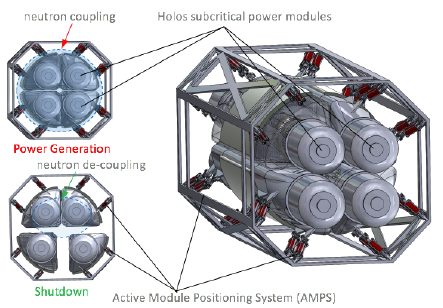
\includegraphics[scale=1]{Figs/holosquad.jpeg}
\caption{Holos Quad generator}
\label{Holosquad}
\end{figure}

\begin{figure}[hbtp]
\centering
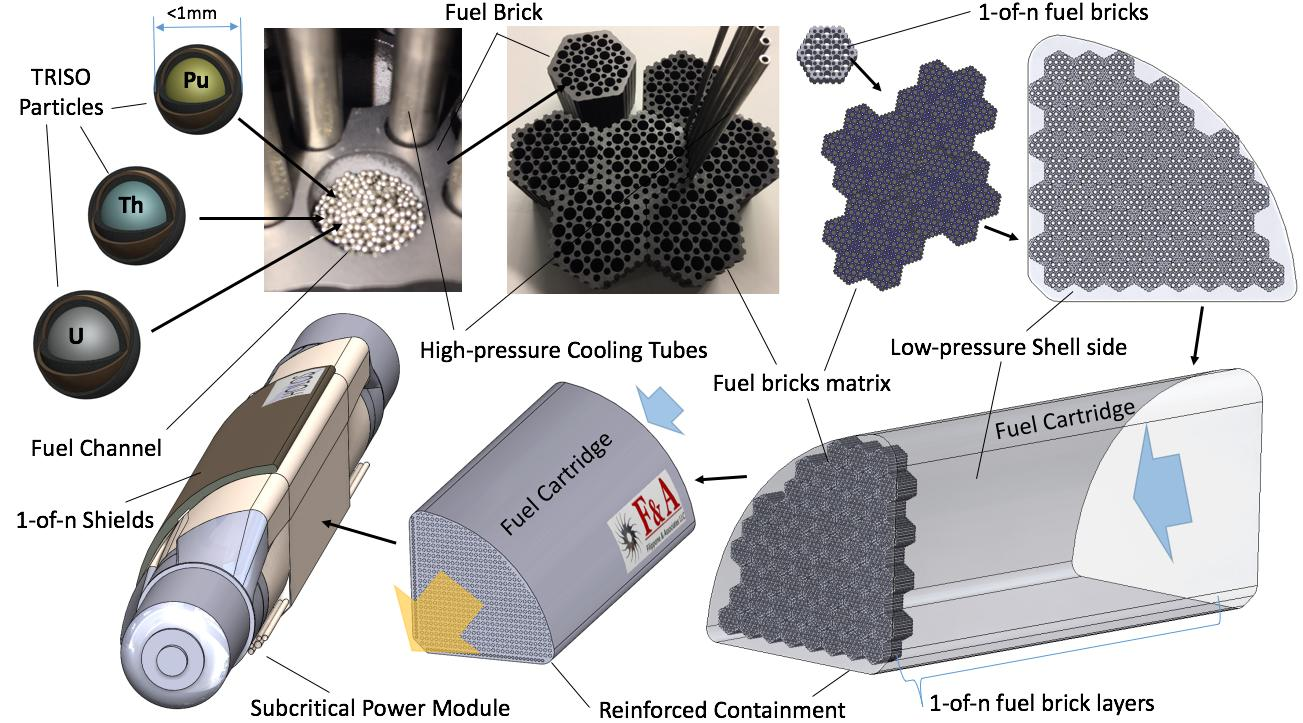
\includegraphics[scale=0.3]{Figs/holosfueldesign.jpeg}
\caption{Holos subcritical assembly design}
\label{Holosdesign}
\end{figure}

\pagebreak

\subsection{Hydromine}
LFR-TL (Transportable Long-life core) is a 15 MWt / 5 MWe lead cooled fast reactor (LFR), with UO2fuel,19.75\% enriched. The coolant is forced circulation lead, inlet/outlet temperature 360/420 $^\circ{}$C. The core lifetime is 15 years. The power conversion is a conventional steam cycle. LFR-AS (Amphora Shape) is a 480 MWt / 200 MWecommercial version of the reactor.

\subsection{Kairos  Power}
KP-FHR is  a  310  MWt  /  140  MWe  fluoride  salt  cooled  high-temperature  reactor  (FHR),  graphite moderated,  pebble  bed  UO2TRISO  fuel  (19.9\%  enriched). The  primary coolant  is  forced  circulation  fluoride  salt (Li2BeF4), system pressure 0.3 MPa, core inlet/outlet temperatures 600/700 $^\circ{}$C. On-line fueling allows for continuous operation, fuel pebbles pass through the core $\sim$ 8 times to achieve burn up to 180 GWd/tHM. The power conversion is a conventional steam cycle.

\subsection{LANL}
MegaPower is a LANL reactor design concept. Table \ref{Megatable} provides important features of MegaPower reactor parameters. More specific design details can be found in the reports \cite{sterbentz_special_2017} and \cite{mcclure_design_2015}. Results of the neutronics and thermal-hydraulics analyses have been published by \gls{INL} and LANL in various reports. Apart from a 5 MWt design, there is an advanced 15 MWt design which uses UN fuel and Na as HP fluid. However, publications are mostly on the first design shown in Figs. \ref{Megadesign} and \ref{Megaoverview}. 

\begin{figure}[hbtp]
\centering
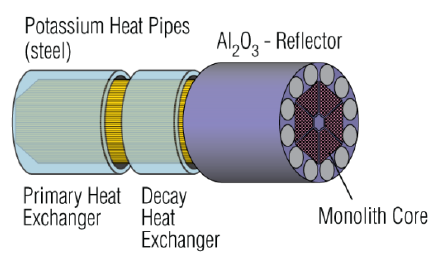
\includegraphics[scale=0.8]{Figs/megacore.jpeg}
\caption{Megapower concept design}
\label{Megadesign}
\end{figure}

\begin{figure}[hbtp]
\centering
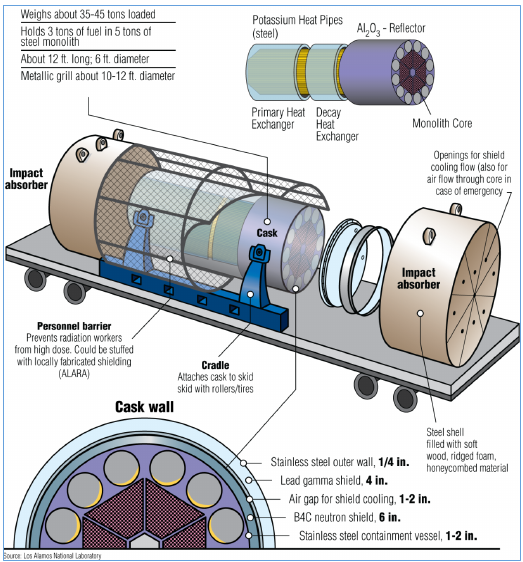
\includegraphics[scale=0.7]{Figs/megacask.jpeg}
\caption{Megapower reactor overview}
\label{Megaoverview}
\end{figure}

\pagebreak
\begin{table} [hbtp]
\begin{center}

\caption{MegaPower Reactor Core Description}
\label{Megatable}
\begin{tabular}{l     l}
\hline 
Design 		&Value \\ 
\hline 
Reactor thermal power&5 MW                                             \\
Reactor electrical power output&2 MW(e)                                       \\
Reactor core orientation&Horizontal                                       \\
Cycle length&5 years                                           \\
Coolant system&Heat pipes                                      \\
Reactor structure&Type 316 Stainless steel monolith    \\
\hline 
Fuel Form&UO2                      \\
Theoretical density&10.96 g/cm$^3$           \\
Percent of theoretical density&96.0\%                   \\
U-235 enrichment&19.75 wt\%             \\
Fuel channel hole outer diameter&1.425 cm               \\
Fuel pellet geometry&Cylindrical              \\
Fuel pellet outer diameter&1.412 cm               \\
Gas gap thickness&0.0065 cm             \\
Fuel rod length&150.0 cm               \\
Fuel-to-fuel pitch&1.60 cm                 \\
Fuel-to-HP pitch&1.60 cm                 \\
Gas&Helium                   \\
Gas pressure&20 atmospheres   \\
Number of fuel rods in-core&2,112                     \\
\hline 
Number of HPs in-core&1,224         \\
HP hole diameter (in-core)&1.575 cm    \\
HP-to-HP pitch&2.7713 cm  \\
HP working fluid&Potassium  \\
HP total length&4.0 m         \\
HP isothermal temperature&675$^\circ{}$C        \\
\hline 
Monolith material&Stainless steel (SS316)       \\
Monolith steel density&8.03 g/cm$^3$                         \\
Monolith edge thickness (HP-to-edge)&2 mm                                 \\
Web thickness between HP-to-fuel holes&0.100 cm                            \\
Web thickness between fuel-to-fuel holes&0.175 cm                            \\
Web thickness between HP-to-edge of block&0.150 cm                            \\
\hline 
Side reflector material&Alumina (Al2O3)       \\
Alumina density&3.9 g/cm$^3$                        \\
Side reflector outer radius&77.85 cm                                 \\
Side reflector radial thickness&21-29 cm                            \\
Top/bottom reflector material&SS316 + BeO                            \\
\hline 
Number of control drums&12       \\
Number of emergency control rods&2       \\
Control material&B4C                        \\
\hline 

\end{tabular}
\end{center}
\end{table}

\pagebreak
\subsection{MicroNuclear}
MsNB  (Micro-Scale  Nuclear  Battery)  is  a  10  MWe  heat  pipe  reactor  (HPR),  cooled  by sodium/potassium heat pipes, molten salt fuel (enrichment undisclosed). The core is molten salt (FLiBe) with dissolved fuel,  with  no  recirculation  outside  of  the  vessel.  The  reactor  can  operate  10  years  without  refueling.  The  power conversion is a Brayton cycle.

\subsection{Moltex Energy}
SSR (Stable Salt Reactor) is 375 MWt / 150 MWe molten salt reactor (MSR), fuel salt 60/40\% NaCl / AcCl3 (enrichment  not  reported). There  is  a  fast  and  thermal  (graphite  moderated)  version. The primary  coolant  is forced circulation 42/10/48\% ZrF4/NaF/KF, melting point 385 $^{\circ}$C. Core inlet/outlet temperature is 525/650 $^{\circ}$C. The molten salt fuel is stationary inside of a fuel pin, arranged as a lattice similar to LWR geometry. Fuel pins are inside of vessel with molten salt coolant. Fuel pins are open and allowed to vent fission gases, such configuration allows for high burnup  due  to  venting  of  fission  gases  and  axially  uniform  burn  due  to fuel salt  mixing. On-line  fueling  allows  for continuous operation. The power conversion is not specified.

\subsection{NuGen}
NuGenEngine  is  1-50  MWe  gas  cooled  reactor  (GCR). Very  little  information  about  this  reactor  is available directly from the company.

\subsection{NuScale}
NuScale micro reactor is a 1-10 MWe heat pipe reactor (HPR). Very little information about this reactor is available directly from the company.

Detailed technical specifications (as seen in Table \ref{Nutable}) related to reactor core design, source term, licensing requirements and safety assessments are given in the NRC web-page \cite{nuscale_chapter_2018-1}. This is the \gls{FSAR} for the SMR design of NuScale. NuScale considers two different micro-reactor concepts \cite{nichol_cost_2019}: one (10-50 MWe) is based on current small modular reactor technology and the other (1-10 MWe) is based on heat pipe reactor technology. The first one is very similar to the SMR. FSAR report  seems quite sufficient by supplying all the details about the plant. 2D and 3D views of the reactor are illustrated in Figs. \ref{Nu2d} and \ref{Nu3d}, respectively. This design can be altered for the $\mu$R concept of NuScale for a nominal electric power of less than 20 MW. There is no detail on the heat pipe design.  \\
In 2018, BWX Technologies was selected to provide manufacturing input. In 2019, Doosan Heavy Industries and Construction and NuScale signed an MOU. 

\begin{table} [htbp]
\begin{center}

\caption{NuScale Reactor Core Description \cite{nuscale_chapter_2018}}
\label{Nutable}
\begin{tabular}{l     l}
\hline 
Design 		&Value \\ 
\hline 
Core diameter (in)			&59.25\\
Active fuel height (in)	&78.74\\

Number of FA 		&  37\\
Rod array   			&17x17\\
Fuel assembly length (in) &  94\\
Fuel assembly pitch (in)	&8.466\\
Fuel rod pitch (in)&0.496\\
Number of spacer grids&5\\
Grid height (in)&1.75\\
Number of Fuel rods&264\\
Number of Guide tubes&24\\
Number of Instrumentation tubes&1\\
\hline 
Number of FR&264\\
Diametrical gap (in)&0.0065\\
Cladding material&M5\\
Cladding outside diameter (in)&0.374\\
Cladding inside diameter (in)&0.326\\
Cladding thickness (in)&0.024\\
Fill gas&helium\\
\hline 
Fuel Pellet Density, \% TD&96\\
Material&UO2 (sintered)\\
Diameter (in)&0.3195\\
Length (in) &0.40\\
\hline 
Number of Control Rod Assemblies&16                              \\
Upper absorber material&boron carbide              \\
Lower absorber material&silver-indium-cadmium \\
Cladding&304 stainless steel      \\
Fill gas&helium                        \\
\hline 
Burnable Absorber Material Type&integral with fuel         \\
Material &gadolinia (Gd2O3 )      \\
Number &Up to 32 per assembly\\
\hline 
Nuclear Design Parameters (for Equilibrium Cycle)\\
Core Average Linear Power (kW/ft)&2.5     \\
Total Heat Flux Hot Channel Factor&1.860  \\
Nuclear Enthalpy Hot Channel Factor&1.386  \\
\hline 
Reactivity Coefficients\\
Doppler temperature coefficient (pcm/F)&-1.4 to -2.25\\
Moderator temperature coefficient (HZP-HFP) (pcm/F)&+6 to -43     \\
Boron coefficient (pcm/ppm)&-10             \\
\hline 
Effective Delayed Neutron Fraction 
and Prompt Neutron Lifetime\\
$\beta_{eff}$ - \gls{BOC}&0.0059\\
$ \beta _{eff}$ - \gls{EOC}&0.0052\\
Prompt lifetime BOC (10-6 seconds)&18.35  \\
Prompt lifetime EOC (10-6 seconds)&-6       \\
\hline 
Boron Concentration (BOC) (ppm)&2000\\
\hline 
*\gls{HZP}, \gls{HFP}
\end{tabular}
\end{center}
\end{table}


\begin{figure}[htbp]
\centering
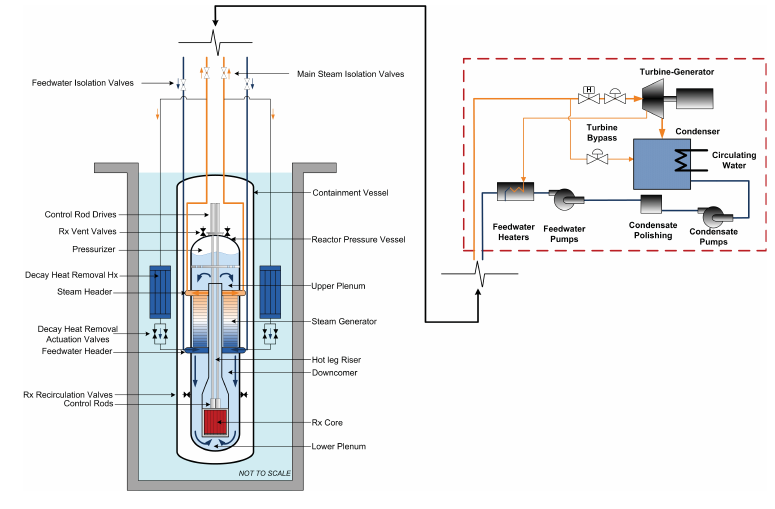
\includegraphics[scale=0.7]{Figs/nuscale2d.jpeg}
\caption{ Two-dimensional schematic of a single NuScale unit}
\label{Nu2d}
\end{figure}

\begin{figure}[htbp]
\centering
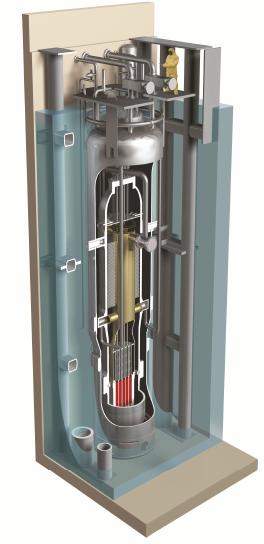
\includegraphics[scale=0.8]{Figs/nuscale3d.jpeg}
\caption{NuScale 3D SMR view}
\label{Nu3d}
\end{figure}

\pagebreak
\subsection{Oklo}
Oklo is working on a Compact Fast Reactor design since 2013. Oklo  is a 2  MWe  heat  pipe  reactor  (HPR),  cooled  by  sodium  heat  pipes,  fast  spectrum,  metallic  fuel (enrichment undisclosed). The reactor is designed to operate purely on natural physical forces, with very few moving parts. The core lifetime is up to 20 years before refueling. Very little information about this reactor is available directly from the company.

Since November 2016, NRC has been engaged in pre-application activities (the docket number - 99902046) with Oklo. Public version of the final safety analysis report of Oklo \cite{oklo_inc._pilot_2018} is not enough for the understanding of the reactor design. Full version has details such as probabilistic risk assessment, release pathway and environmental impact but was closed to public access. Even company web site is unreachable. The company is now making collaboration with ANL and INL. 

\subsection{Starcore}
The StarCore technical data is acquired directly from the vendor website and summarized in Table \ref{startable} below. In terms of size and basic technical characteristics, the reactor, illustrated in Fig \ref{Starcore}, is similar to HTR-10, a prototype pebble bed modular reactor built and operated in China, and HTTR, a 30 MWth experimental gas cooled reactor in Japan.

HTGR reactor with 2 reactor units per standard plant is embedded 15m underground in \gls{UHSC} silos. The reactors are installed in silos 57 meters deep (as seen in Fig. \ref{Starview}) and 13 meters in diameter, made from double-walled high performance concrete with a steel canister silo at the base.  TRISO fuel compacts supplied by BWX Technologies. StarCore is fully automated and has only two operating states: Load Following and Shutdown.

\begin{figure}[htbp]
\centering
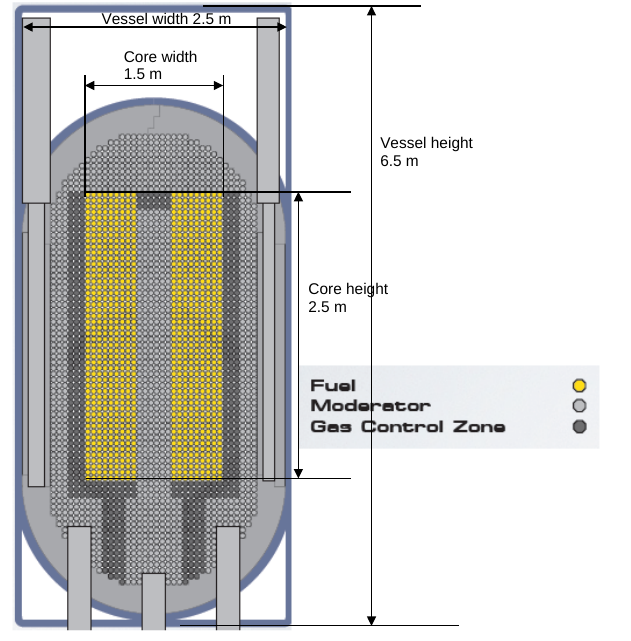
\includegraphics[scale=0.5]{Figs/starcorereactor.jpeg}
\caption{StarCore reactor core}
\label{Starcore}
\end{figure}

\begin{figure}[htbp]
\centering
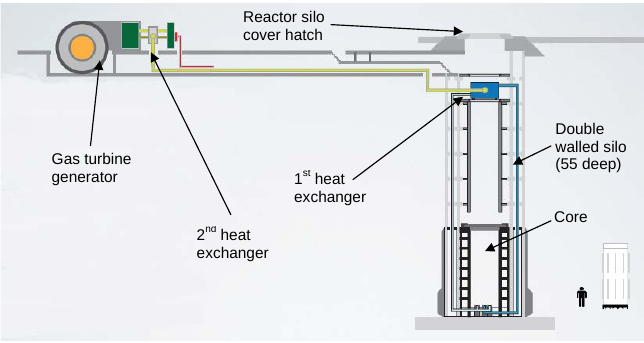
\includegraphics[scale=0.7]{Figs/starcoreview.jpeg}
\caption{Side view of Starcore}
\label{Starview}
\end{figure}

\begin{table} [ht]
\begin{center}

\caption{StarCore reactor design}
\label{startable}
\begin{tabular}{l l}
\hline 
Design 		&Value \\ 
\hline 
Core Diameter (m) 		&1.5 \\ 
Core Height (m) 		&2.5 \\ 
Refueling (y)		&  5 (off-site)\\ 
Fuel		&UCO TRISO Pebbles \\ 
Enrichment (\%)		&$<$20 \\ 
Number of fuel pebbles		&26,800 \\ 
Number of TRISO particles per pebble		&2,000 \\ 
Pebble fuel core diameter (mm)		&60 \\ 
Fuel element geometry & Truncated cuboctahedron\\ 
Cladding material & Silicon carbide \\ 
Primary side coolant 	&Helium \\ 
Core outlet temp ($^\circ{}$C) 	&850 \\ 
Core operating pressure (MPa)	&7.5 \\ 
Secondary side coolant	&Nitrogen \\ 
Secondary side operating pressure (MPa)	&6.8 \\ 
\hline 

\end{tabular}
\end{center}
\end{table}

\pagebreak
\subsection{Urenco}
The concept design, namely U-battery, has been made by the Universities of Manchester, Dalton Institute (UK) and Technology University of Delft (Netherlands). There is strong desire to operate the reactor by 2026. Main design parameters \cite{ding_design_2011} are tabulated in Table \ref{Utable}. A 3D view and core layout of the reactor are displayed in Figs. \ref{u3d} and \ref{ucore}. 

The coolant is pressurized He, the secondary side is cooled by nitrogen. It provides up to 750 $^\circ{}$C process heat. The power conversion is not specified.

\begin{table} [htbp]
\begin{center}

\caption{U-battery design}
\label{Utable}
\begin{tabular}{l l l}
\hline 
Design 		&10 MWe &20 MWe\\ 
\hline 
Reflector composition & BeO          &  Graphite\\
Control rods (\#) & 4                        &  6 \\
Fuel Blocks (\#) & 6*4                     & 30*4 \\
Enrichment (\%) & 20                      & 17  \\
Fuel life time (a)&  5                       & 10  \\
Fuel block dimension (cm) & 36*80 &  36*80 \\
Fuel mass (kg) & 208                     &   1.040\\
Burn-up (MWd/kg HM)  & 88           &   70 \\
\hline 
Outer diameter (cm)             &   180  &  370   \\
Vessel thickness (mm)        &   $<$100       & 100   \\
Reactor core diameter (cm)  &   108     &  252  \\
Reflector thickness (cm)      &   20 (BeO)    &29    \\
Insulation thickness (cm)     &   5 (SiC fiber)     & 10 (SiC fiber)   \\
Barrel thickness (cm)           &    2   & 2    \\
Gap thickness (cm)             &    5  &  5  \\
\hline 
Core Height (cm)          & 320         & 320 \\
Top reflector (cm)         &  20 (BeO)&50  \\
Bottom reflector (cm)    &  20 (BeO)& 50 \\
Top plenum (cm)          &20            &20  \\
Bottom plenum (cm)     &  50          &50  \\
Top insulation (cm)       &30           &30 \\
Bottom insulation (cm)  &  60         &60 \\
Core support plate (cm) &  10         &15  \\
Support structure (cm)  &   60         &60  \\
Vessel height (cm)       & 590         &655  \\
\hline 
BeO mass (kg) &    7.900       &0  \\
Graphite mass (kg) &   8.100        & 70.000  \\
Flask inner diam (cm)& 180       & - \\
Flask inner height (cm)& $<$500         & - \\
\hline 

\end{tabular}
\end{center}
\end{table}


\begin{figure}[htbp]
\centering
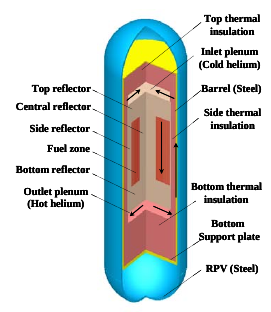
\includegraphics[scale=1]{Figs/ubattery3d.jpeg}
\caption{ 3D reactor configuration of U-battery}
\label{u3d}
\end{figure}

\begin{figure}[htbp]
\centering
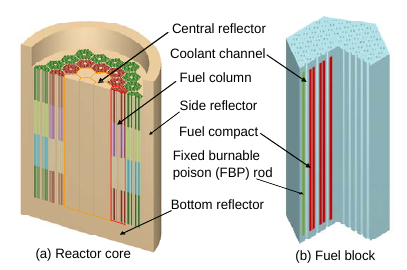
\includegraphics[scale=1]{Figs/ubatterycore.jpeg}
\caption{ Core and fuel block of U-battery}
\label{ucore}
\end{figure}


\pagebreak
\subsection{Terrestrial Energy}
Integral Molten Salt Reactor (IMSR) is 400 MWt / 195 MWe molten salt reactor (MSR), graphite-moderated, uranium salt fuel (~5\% enriched). The primary coolant is forced circulation fluoride salt with dissolved fuel, system pressure ~0.4 MPa (hydrostatic), core inlet/outlet temperatures 660/700 $^\circ{}$C. The IMSR is a sealed reactor vessel with integrated pumps, heat exchangers and shutdown rods all mounted inside a single vessel. The sealed core-unit is replaced at the end of its useful service life (nominally 7 years). The power conversion is a conventional steam cycle.

\subsection{USNC}
MMR (Micro Modular Reactor) a 15 MWt/ 5 MWe gas cooled reactor (GCR),  graphite moderated, TRISO fuel (enrichment 9-12\%) in  a  prismatic  graphite block. The coolant is natural convection helium, the intermediate heat transfer loop is molten salt, outlet temperature 640 $^\circ{}$C. The core lifetime is 20 years, with no refueling. The power conversion is not specified.

\pagebreak
\subsection{X-energy}
X-energy company provides various reactor designs ranging from 600 MWt to 30 MWt, called Pebble Bed Fuel Reactor. The main microreactor design is ST-OTTO (referring to Fig.  \ref{xo}) which produces 30-48 MWt power. But the design details are not open to the public. I think the design is very identical to the design of 200 MWt, as presented in Table \ref{xtable} except for the reactor size and fuel type. Th-based fuel is under consideration for the use in TRISOs. 

\begin{table} [ht]
\begin{center}

\caption{ X-energy design}
\label{xtable}
\begin{tabular}{l l}
\hline 
Design 		&Value \\ 
\hline 
RPV diameter (m) 		&4.88 \\ 
RPV height (m) 		&20 \\ 
Refueling		&Online fuel loading  \\ 
	&175 fresh pebbles/day \\ 
Fuel		&UCO TRISO Pebbles \\ 
Enrichment (\%)		&15.5 \\ 
Number of fuel pebbles		&220,000 \\ 
Number of TRISO particles per pebble		&18,000 \\ 
Pebble fuel core diameter (mm)		&50 \\ 
Pebble diameter (mm)	&60 \\ 
Number of passes		&6\\ 
Final burnup (GWd/tHM)		&160 \\ 
Burnable poison		&no \\ 
Power density (MW/m$^3$)		&4.8 \\ 
UCO TRISO kernel diameter (mm)	&0.425 \\ 
Porous Carbon Buffer thickness (mm)	&0.095 \\ 
Inner Pyrolytic Carbon Layer thickness (mm) 	&0.04 \\ 
Silicon Carbide Layer thickness (mm)	&0.035 \\ 
Outer Pyrolytic Carbon Layer thickness (mm)	&0.04 \\ 
Core Inlet temp ($^\circ{}$C)	&259 \\ 
Core Outlet temp ($^\circ{}$C) 	&750 \\ 
Core Inlet Pressure (MPa)	&6 \\ 
Core Outlet Pressure (MPa)	&5.84 \\ 
\hline 

\end{tabular}
\end{center}
\end{table}

\begin{figure}[hbtp]
\centering
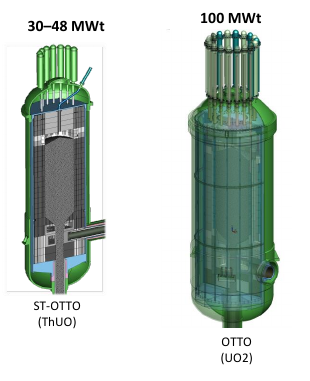
\includegraphics[scale=0.97]{Figs/xoverview.jpeg}
\caption{X-energy micro-reactor overview}
\label{xo}
\end{figure} 

\subsection{Westinghouse}
Full design details have not been revealed yet to the public; only general information is given by the company. However, general characteristic of eVinci is a 5 MWt / 2 MWe heat pipe reactor (HPR), cooled by sodium heat pipes, TRISO fuel (19.75 \% enriched) in  a  solid graphite block  core. It  can  produce  up  to  600 $^\circ{}$C  process  heat, the  waste  heat  is  rejected  to  the atmosphere.  The  core lifetime is 10 years.  It  is  factory  built,  assembled,  fueled,  and  tested, and transported to  the deployment site. The power conversion is not specified.

Several academic studies, most of them eVinci-like, can be found in the literature. Recently, two papers, \cite{hong_thermal_2019} and \cite{wright_phenomena_2019}, have been published in 18th \gls{NURETH} conference. Those are not available for now but reaching them somehow would be valuable. Westinghouse is planning to finalize the current design of eVinci by 2022, testing by 2023 and commercializing by 2025. Hernandez et al. \cite{hernandez_micro_2019} performed a series of calculations in eVinci-like (not eVinci) for natural resource utilization, burnup analyses, waste management and environmental impacts. The details of eVinci design obtained from the documents published by Westinghouse are presented in Table 3. Reactor core configuration and 3D design representation are given in Figs. \ref{eVincidesign} and \ref{eVincioverview}.

\begin{table} [ht]
\begin{center}

\caption{eVinci design parameters}
\begin{tabular}{l  l  l}
\hline
Design 		&Value (from Westinghouse reports) 		& Value (other) \cite{hernandez_micro_2019}\\ 
	& 	\cite{iaea_advances_2018};\cite{levinsky_westinghouse_2018};\cite{yan_technology_2020};\cite{arafat_evinci_2019} 	&  \\ 
\hline
Core Diameter (in) 		&59.06 		&  \\ 
Monolith materials 		& 		& Type-316 SS	\\ 
Refueling (years) 		&Up to 10 		&  \\ 
Fuel 		&UN/U-Mo 		& 	 \\ 
Fuel Pellet Density, \% TD 		&96 		&  \\ 
Enrichment (\%) 		&19.75 		&  \\ 
Fuel channel radius (in) 		& 		& 0.281 \\ 
Number of fuel channels 		&378 (1 MWth), 4219 (14 MWth)		& 2112 (5 MWth) \\ 
Reflector material 		&		& BeO\\ 
\gls{HP} channel radius (in) 		&		& 0.298\\ 
Number of HP channels 		& 		& 1224\\ 
HP to HP web thickness (in) 		& 		& 0.039\\ 
Fuel to fuel web thickness (in) 		& 		& 0.059\\ 
HP total length (ft) 		&		& 13.12\\ 
HP fluid 		&Na/K		& \\ 
HP fluid temperature (K) 		&920 		& \\ 
\hline

\end{tabular}
\end{center}
\end{table}

\begin{figure}[hbtp]
\centering
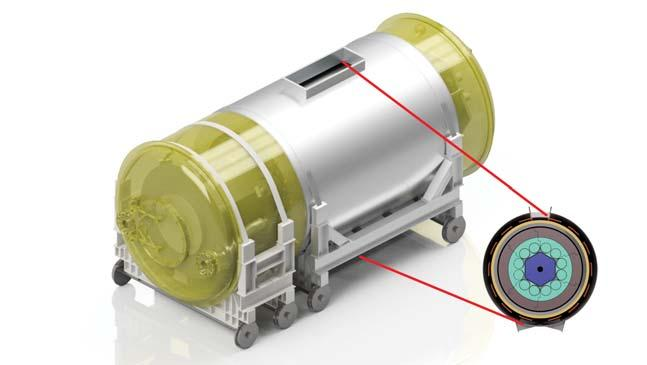
\includegraphics[scale=0.5]{Figs/evincicore.jpeg}
\caption{eVinci Core Configuration}
\label{eVincidesign}
\end{figure}

\begin{figure}[hbtp]
\centering
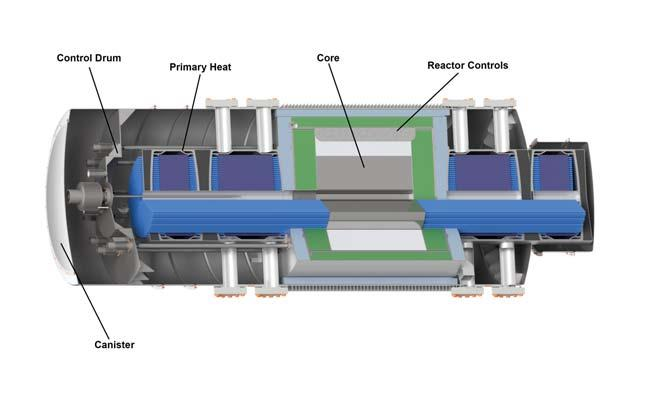
\includegraphics[scale=0.5]{Figs/evinciover.jpeg}
\caption{eVinci Micro Reactor Overview}
\label{eVincioverview}
\end{figure}

\pagebreak


\pagebreak
\section{Site Requirements}

In a White Paper \cite{nrc_staff_population-related_2019} on the “Population-Related Siting Considerations for Advanced Reactors”, two primary issues were identified for the possible deployment of advanced reactors and the NRC’s current siting requirements. The first issue is that population density should not exceed 500 persons per square mile (ppsm) out to a distance of 20 miles from a reactor site. The second issue is the use of SMRs for remote communities or smaller grids with relatively small but concentrated populations that would be near a reactor site. Due to the reduced risks and radiological releases from advanced reactor designs, the NRC is revising the existing guidance on population density.  For that purpose, the NRC suggests four options:

Option-1: Same as the siting requirements of LWRs, with no changes to the current population-related siting regulations or the existing guidance. Fig. \ref{rprox} shows the NRC’s current siting requirements. 

Option-2:  No changes in NRC regulations; however, the staff would revise the population-related guidance to include provisions for advanced reactor designs and more specifically for SMRs.

Option-3: Similar to Option 2 except that the criteria are directly related to estimates of radiological consequences from design-specific events rather than a general correlation of offsite doses to radionuclide inventories or power level. 
The following three cases involving possible offsite consequences from design-basis events and beyond-design-basis events illustrate the limitations on populations near an advanced reactor under Option 3:

1. In the first case for possible advanced reactor designs, the potential offsite consequences of some beyond-design-basis events are calculated to approach 25 rem
over the course of the event.

2. The second case involves an advanced reactor design for which all design-basis events and beyond-design-basis events are calculated to result in doses to an individual at the site boundary of less than 25 rem over the duration of the event. However, for this case, the calculation of some design-basis events or beyond-design-basis events results in offsite doses exceeding 1 rem over the month following the event. 

3. In the third case, the potential consequences from all design-basis and beyond-design-basis events are estimated to be below 1 rem for the month following the event for an individual at the site boundary.

Option-4: Calls for the NRC staff to develop societal risk measures for assessing specific advanced reactor designs at specific sites. 



\begin{figure}[hbtp]
\centering
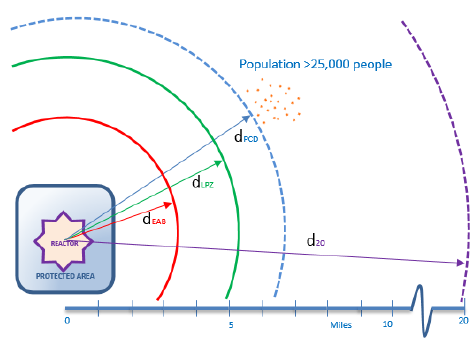
\includegraphics[scale=0.7]{Figs/reactorproximity.jpeg}
\caption{Reactor Proximity to Population Centers}
\label{rprox}

\flushleft
d$_{EAB}$: exclusion area boundary (EAB) radial distance\\
d$_{LPZ}$: low population zone (LPZ) radial distance\\
d$_{PCD}$: population center distance (PCD) to the nearest boundary of a densely populated center\\
d$_{20}$: 20 mile outward radial distance \\
EAB: radial distance based on the 25 rem criteria for any 2 hour period\\
LPZ: radial distance based on the 25 rem criteria during the entire period of the radioactive cloud passage\\
PCD: radial distance from the reactor to the nearest boundary of a densely populated center at least 1 1/3 that of the outer boundary of the LPZ\\
Population Density: the staff also considers the population density of 500 persons per square mile out to 20 miles
\end{figure} 

\pagebreak
\section{Source Term}
For licensing existing operating reactors a mechanistic source\footnote{Mechanistic Source Term: A source term that is calculated using models and supporting scientific data that simulate the physical and chemical processes that describe the radionuclide inventories and the time-dependent radionuclide transport mechanisms that are necessary and sufficient to predict the source term.}
 is used for the transport of the fission products from the fuel through the reactor coolant system, through all holdup volumes and barriers, taking into account mitigation features, and into the environment. Such a method method to determine accident dose is also under consideration for microRs.  \\
 
The source term is expressed as\\
ST(S$_{i}$, RN$_{j}$, t) = I(RN$_{j}$).F(S$_{i}$, t).MR(S$_{i}$, RN$_{j}$, t).PSR(S$_{i}$, RN$_{j}$, t).LPF(S$_{i}$, RN$_{j}$, t)\\
where,\\
ST(S$_{i}$, RN$_{j}$, t) - Source term as a function of the accident scenario (Si), radionuclide class (RNj), and timing (t)\\
I(RN$_{j}$) - Inventory \\
F(S$_{i}$, t) -Fuel damage\\
MR(S$_{i}$, RN$_{j}$, t) - Matrix release\\
PSR(S$_{i}$, RN$_{j}$, t) - Primary system release\\
LPF(S$_{i}$, RN$_{j}$, t) - Leak path factor\\

As tabulated in Table \ref{inputandsource}, inputs that used in the source term calculation may come from experiments or other computer codes. A general source term analysis comprises transient scenario modeling, fuel pin radionuclide distribution, failed pin radionuclide release, radionuclide bubble transport, offsite dispersion analysis and containment region analysis. Some of them can, however, be eliminated or new ones can be added depending on which micro-reactor is to be chosen. As an example, the micro-reactor design does not include any spent fuel storage, thus the source term would not. \\

\begin{table} [ht]
\begin{center}

\caption{ Inputs used in the source term calculations and their sources}
\label{inputandsource}
\begin{tabular}{l l}
\hline 
Input 		&Source \\ 
\hline 
FP inventory 		&SCALE\\ 
FP diffusion coefficients 		&Experiments and analysis (e.g., DOE tools) \\ 
Core power shape		&Radial/Axial profiles (e.g., SCALE or vendor data)  \\ 
Fuel particle failure rate response surface \\
(function of temperature and burnup)	&Experiments/other codes (e.g., DOE tools) \\ 
Dust generation, lift-off, and FP adsorption on dust \\
(impact of aerosol growth, shape factor, etc.)	& Experiments/Historical data and other codes\\ 
FP release under accident conditions \\including air/water ingress 	&Experiments \\ 
FP speciation and interaction \\with graphite and other structures &Experiments  \\ 
\hline 

\end{tabular}
\end{center}
\end{table}

MicroRs have significantly lower source terms (about 1\% of typical 1000 MWe LWR) due to their reduced fuel inventory and passive safety features. A reduced source term would facilitate siting SMRs in locations where nuclear plants have not been traditionally sited.\\\\
For the source term analysis of a selected micro-reactor design, phenomena and release paths of accident scenarios first need to be identified. Eventhough pathways for some advanced reactors (i.e., HTGR, \gls{SFR}, MSR) illustrated in Fig. \ref{pathway} are known  \cite{inl_htgr_2010}, there are on-going discussions in the NRC on the evaluation of the source term of micro-reactors; it is expected to come to a conclusion on the licencing issues including the source term by the end of this year (estimated). 

\begin{figure}[hbtp]
\centering
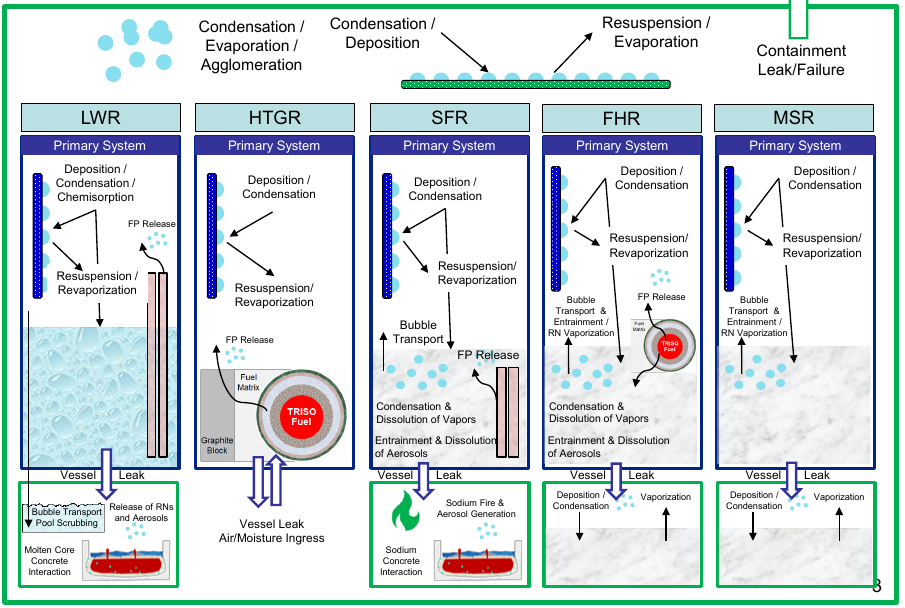
\includegraphics[scale=0.6]{Figs/pathway.jpeg}
\caption{Pathway for radioactive release for several reactor types}
\label{pathway}
\end{figure}

There is a possibility to make an assumption for the pathway identification of the micro-reactors. We can use the same or modified pathways of the existing reactors, accepted by the NRC, for the analogy to the selected micro-reactor design. \\

A recent document by the NRC \cite{nrc_staff_nrc_2019} has published for the source term calculations of non-LWR reactors.
The method for the source term calculation recommended by the NRC is given in Fig. \ref{sourceterm}. The method to be applied changes with the type of the reactor. In any cases, as a code system, SCALE calculates radioactive material composition for the licensed current and advanced reactors and provides necessary data to MELCOR. MELCOR, system accident analysis code, produce the source term for the defined design-basis accidents. And then, for probabilistic offsite consequence analysis bounded by the calculated source term, MACCS code needs to be utilized. The code is capable of evaluating the Level 3 \gls{PRA} including the radionuclide release, atmospheric transport, meteorology, protective actions, site data, dosimetry, health effects, economic factors, and so forth. Design-specific and site-related issues must be input to the code.  Meteorological statistics (i.e., day and night temperatures, magnitude and direction of the wind, tornados, flooding level), topographical data and population density and distribution, habitat of the animals and the location of the endemic plants are to be recorded. \\

The methodology and the results on the source term calculations are presented in detail in the relevant documents of NuScale \cite{nuscale_chapter_2018-1} and eVinci \cite{maioli_westinghouse_2019}.According to the NuScale, the potential radionuclide source term associated with a severe accident is much smaller (5\%) than that associated with a 1000 MWe design. This value is 1\% for eVinci. 

\begin{figure}[hbtp]
\centering
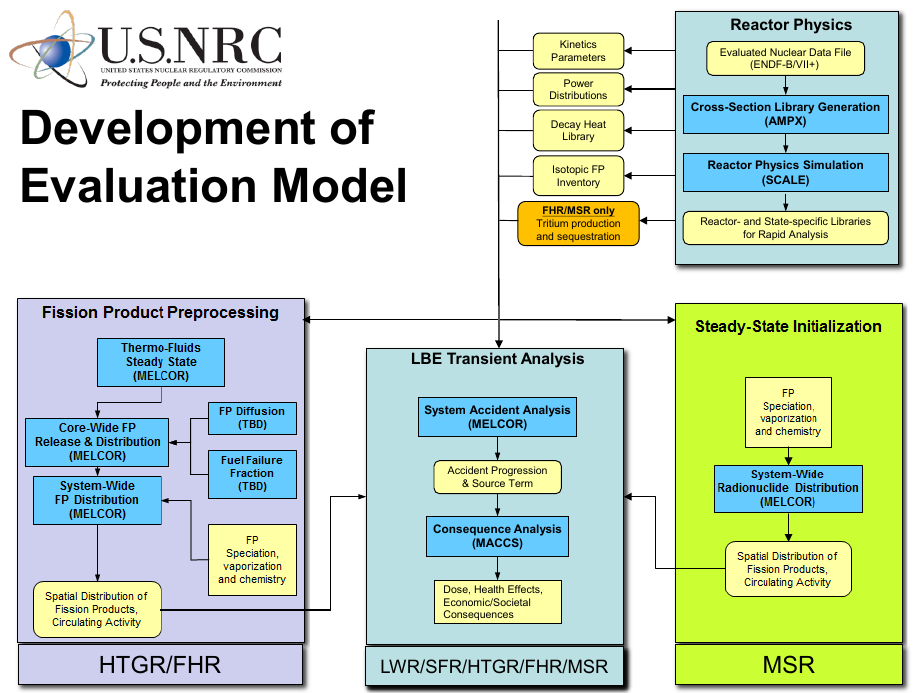
\includegraphics[scale=0.6]{Figs/sourceterm.jpeg}
\caption{Source term evaluation model}
\label{sourceterm}
\end{figure}

\subsection{HTGR}
Pathway for HTGR is given in the reference  \cite{inl_htgr_2010}. There is a generic pathway almost for all HTGRs. NRC evaluation model for HTGRs is displayed in Fig. \ref{sourceterm}. Source term calculation for HTGRs is given in Fig.  \ref{htgrsourceterm}. 

\begin{figure}[hbtp]
\centering
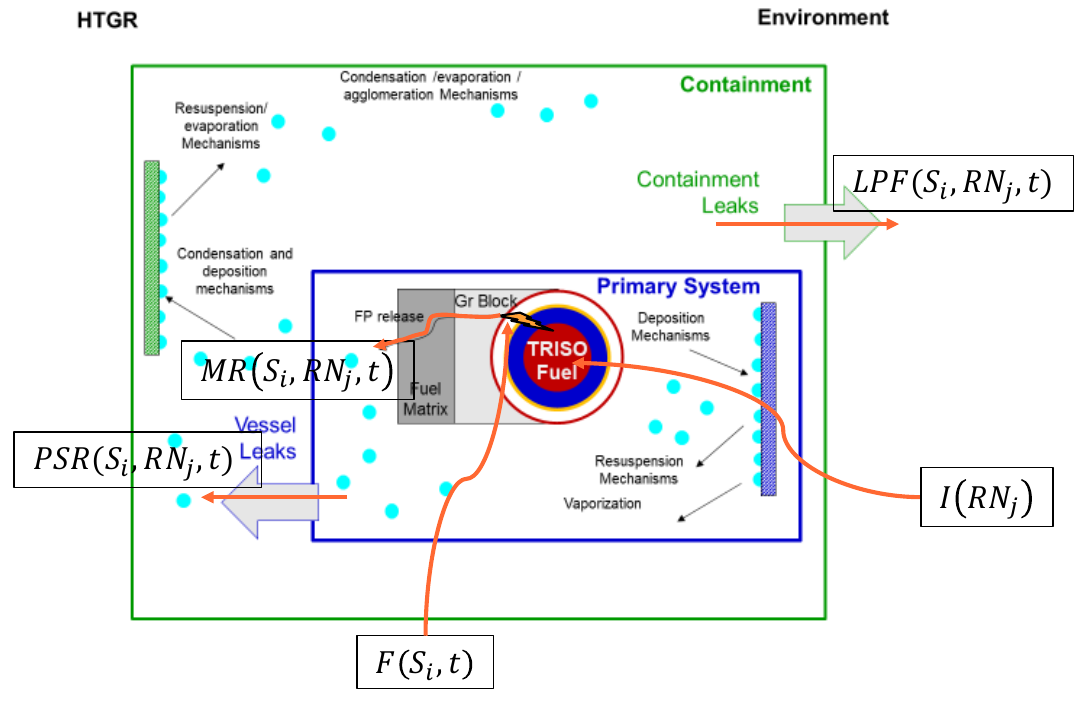
\includegraphics[scale=0.5]{Figs/htgrsourceterm.jpeg}
\caption{Source term calculation for HTGRs}
\label{htgrsourceterm}
\end{figure}

\subsection{Heat Pipe Reactor}
In contrast to HTGRs, pathways for the radioactive material release from the heat pipe reactors are completely unknown. However, source term evaluation model is very similar to HTGRs once the pathway of HPRs is defined.  





\pagebreak
\section{Licencing Procedure}
For the licensing of the research reactors, below documents are critical:

1. Guidelines for Preparing and Reviewing Applications for the Licensing of Non-Power Reactors: Standard Review Plan and Acceptance Criteria (NUREG 1537, Part 2).

2. Guidelines for Preparing and Reviewing Applications for the Licensing of Non-Power Reactors: Format and Content (NUREG 1537, Part 1). 


https://www.nrc.gov/reading-rm/doc-collections/nuregs/staff/sr1537

A reference document \cite{nichol_roadmap_2018} has discussed  the micro-reactor from the various acpects inculding waste management, fuel supply and action plans.


\section{Safety Assessment}
This part is going to be discussed later but will include accident scenarios including design-basis that a nuclear facility must be designed and built to withstand, and beyond design accidents that are possible but were not fully considered in the design process.

\section{Discussion on the Report}

Considering available data of the interested reactors given in Section \ref{sec:reactors}, full core modeling capabilities are presented in Table \ref{table:feasiblity}. it should be taken into account that desing details of the reactor to be selected can be gathered from the corresponding vendor. What should be the criteria for the selection of the micro-reactor?

1. according to reactor type

2. according to NRC review

3. 

\begin{table} [ht]
\begin{center}

\caption{Full core modeling}
\label{table:feasiblity}
\begin{tabular}{|l|l|l|l|l|l|l|l|l|l|}
\hline 
Design 		&eVinci 		& Holos		&MegaPower 	& NuScale		& Oklo 		& Starcore		& U-battery 	 & MMR	& Xe-100 \\ 
\hline 
$\times$ or 	$\surd$ 		&  $\times$		& $\surd$		& $\surd$ 	&   $\surd$		&  $\times$		& $\surd$	&  $\surd$ 	&  $\surd$	&  $\surd$ \\ 
\hline 

\end{tabular}
\end{center}
\end{table}

\pagebreak
\section{Conclusion}

\pagebreak

\bibliography{MicroReactor}


\end{document}
